% Waterfall chart: ISA ablation — cumulative instret reduction per extension
% §9.2.1 — HQC-128 Decaps, Spike ISS
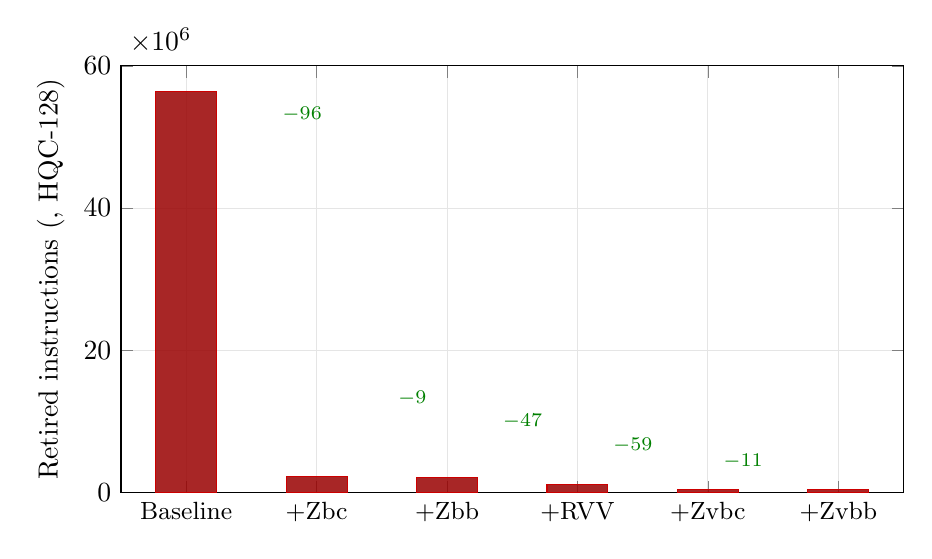
\begin{tikzpicture}
\begin{axis}[
    ybar stacked,
    bar width=22pt,
    width=0.95\textwidth,
    height=7cm,
    ylabel={Retired instructions (\Decaps, HQC-128)},
    symbolic x coords={Baseline, {+Zbc}, {+Zbb}, {+RVV}, {+Zvbc}, {+Zvbb}},
    xtick=data,
    x tick label style={font=\small},
    ymin=0,
    ymax=60000000,
    scaled y ticks=base 10:-6,
    ytick scale label code/.code={$\times 10^6$},
    nodes near coords style={font=\tiny, /pgf/number format/fixed},
    legend style={at={(0.98,0.95)}, anchor=north east, font=\small},
    every axis plot/.append style={fill opacity=0.85},
    grid=major,
    grid style={gray!20},
]

% Stacked bars showing remaining instret at each stage
% Data: ref_scalar baseline → karatsuba_zbc → +Zbb → karatsuba_rvv → karatsuba_zvbc → +Zvbb Keccak
% Baseline (no crypto extensions): ref_scalar ≈ 56.4M (decaps)
% +Zbc (karatsuba_zbc): 2.06M decaps
% +Zbb: 2.06M → (Zbb saves ~10% Keccak portion)
% +RVV recomposition: karatsuba_rvv ≈ 1.08M
% +Zvbc leaves: karatsuba_zvbc ≈ 444K
% +Zvbb Keccak: karatsuba_zvbc+zvbb ≈ 394K

\addplot[fill=red!60!black, draw=red!80!black] coordinates {
    (Baseline, 56442467)
    ({+Zbc}, 2263224)
    ({+Zbb}, 2060797)
    ({+RVV}, 1094531)
    ({+Zvbc}, 444324)
    ({+Zvbb}, 394225)
};

\end{axis}

% Annotations: delta percentages between bars
\node[font=\scriptsize, text=green!50!black] at (2.3, 4.8) {$-\pct{96}$};
\node[font=\scriptsize, text=green!50!black] at (3.7, 1.2) {$-\pct{9}$};
\node[font=\scriptsize, text=green!50!black] at (5.1, 0.9) {$-\pct{47}$};
\node[font=\scriptsize, text=green!50!black] at (6.5, 0.6) {$-\pct{59}$};
\node[font=\scriptsize, text=green!50!black] at (7.9, 0.4) {$-\pct{11}$};

\end{tikzpicture}
